\documentclass[12pt,a4paper]{article}
\usepackage[utf8]{inputenc}
\usepackage[margin=1in]{geometry}
\usepackage{amsmath}
\usepackage{amssymb}
\usepackage{amsthm}
\usepackage{booktabs}
\usepackage{float}
\usepackage{hyperref}
\usepackage{natbib}
\usepackage{setspace}
\usepackage{tikz}
\usepackage{adjustbox}
\usetikzlibrary{positioning, arrows.meta, shapes}

\onehalfspacing

\title{Measuring and Optimizing Advertising Incrementality with Ghost Ads}
\author{}
\date{}

\begin{document}

\maketitle

\begin{abstract}
Advertising platforms face a fundamental challenge: distinguishing correlation from causation in user behavior. We present ghost ads methodology for measuring incremental effects and demonstrate how these measurements enable optimal resource allocation. Through mixed-integer linear programming on synthetic data calibrated to marketplace conditions, we show that causal optimization achieves 36-90\% higher incremental return on ad spend compared to correlation-based methods across bidding, ranking, frequency capping, and eligibility decisions. The key insight is that baseline purchase probability and treatment effects exhibit strong negative correlation—users who would convert organically show minimal lift from advertising. By identifying and targeting high-lift users, causal methods dramatically improve platform economics while reducing wasted impressions.
\end{abstract}

\section*{The Incrementality Problem\footnote{In this note, "incrementality" means the average treatment effect on the treated: the expected increase in purchase outcomes among users who actually receive an impression compared with what those same users would have done without the ad.}}

The main problem in measuring advertising effectiveness is telling the difference between correlation and causation. If you compare users who saw ads to users who didn't, you're mixing together people who would have bought anyway with people who \textit{only bought because of the ad}. 

People in hospitals are more likely to die, but hospitals don't cause death in people; it is just that sick people seek hospitals. In the same way, people who really want to purchase something are more likely to see and click on ads, but that doesn't necessarily mean the ads caused them to buy.

\begin{itemize}
\item When a user clicks an ad and buys something, the ad might have convinced them to buy, or they might have already planned to buy and just used the ad to find the product.
\item Users who see more ads are different from users who don't, both in ways we can see (like search history and browsing patterns) and in ways we can't see (e.g. how much they wanted to buy in the first place).
\end{itemize}

\begin{figure}[H]
\centering
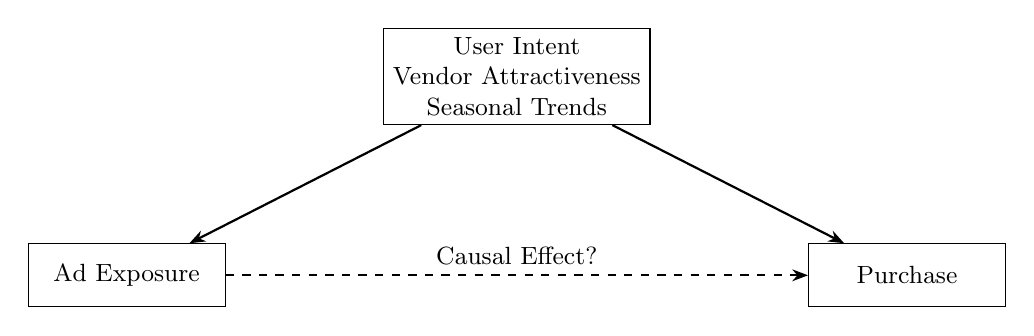
\begin{tikzpicture}[
    node distance=2.5cm,
    every node/.style={font=\small,align=center},
    arrow/.style={-{Stealth[length=2mm]}, thick}
]
    \node (intent) [draw, rectangle, minimum width=2.5cm, minimum height=0.8cm] {User Intent \\ Vendor Attractiveness \\ Seasonal Trends};
    \node (ad) [draw, rectangle, below left=1.5cm and 2cm of intent, minimum width=2.5cm, minimum height=0.8cm] {Ad Exposure};
    \node (purchase) [draw, rectangle, below right=1.5cm and 2cm of intent, minimum width=2.5cm, minimum height=0.8cm] {Purchase};

    \draw [arrow] (intent) -- (ad);
    \draw [arrow] (intent) -- (purchase);
    \draw [arrow, dashed] (ad) -- node[above, sloped] {Causal Effect?} (purchase);
\end{tikzpicture}
\caption{User intent affects both ad exposure and purchase decisions.}
\label{fig:dag}
\end{figure}

What we really want to know is the persuasive effect of the ad—the purchases that would not have happened without the ad. That is the value to the marketplace, and the real reason why vendors are ready to pay for ads. But we can't see measure that directly from correlations.

\subsection*{A Simple Example}

Suppose, in reality, the ad actually increases purchase rates by 5 percentage points for everyone. Say you have two types of users: type A high-intent users (80\% would buy anyway and show signs) and type B low-intent users (10\% would buy anyway and show signs of disinterest). The ad system, powered by targeting algorithms, shows ads to 90\% of type A users and only 10\% of type B users (it is doing its job!).

Table \ref{tab:confounding_example} shows what happens with 1,000 users (500 type A, 500 type B).

\begin{table}[H]
\centering
\caption{Numerical Example of Confounding Bias}
\label{tab:confounding_example}
\begin{tabular}{lcccc}
\toprule
User Type & Count & Ad Exposure & Purchase Rate & Purchases \\
\midrule
\multicolumn{5}{l}{\textit{Type A Users (Baseline 80\%)}} \\
\quad Exposed to Ad & 450 & Yes & 85\% & 382.5 \\
\quad Not Exposed & 50 & No & 80\% & 40.0 \\
\addlinespace
\multicolumn{5}{l}{\textit{Type B Users (Baseline 10\%)}} \\
\quad Exposed to Ad & 50 & Yes & 15\% & 7.5 \\
\quad Not Exposed & 450 & No & 10\% & 45.0 \\
\addlinespace
\multicolumn{5}{l}{\textit{Aggregate Observed Data}} \\
\quad All Exposed & 500 & Yes & 78.0\% & 390 \\
\quad All Not Exposed & 500 & No & 17.0\% & 85 \\
\addlinespace
\multicolumn{5}{l}{\textit{Naive Estimate}} \\
\quad Difference & & & 61.0 pp & \\
\addlinespace
\multicolumn{5}{l}{\textit{True Causal Effect (Assumed Constant)}} \\
\quad Within Type A & & & 5.0 pp & \\
\quad Within Type B & & & 5.0 pp & \\
\bottomrule
\end{tabular}
\end{table}

If you compare the two groups, you see 78\% of ad viewers bought versus 17\% of non-viewers. That's a 61 percentage point difference. But the real ad effect is only 5 percentage points. The bias gets worse when targeting is better. If only type A users saw ads, you'd measure a 75 percentage point difference when the real effect is still 5 percentage points. If targeting is random, there's no bias. But good ad systems are \textit{not random}. The better your targeting, the harder it is to trust correlations between ad-impressions and purchases.

\subsection*{What Causes This Problem in Marketplaces}

Even the best ad-system does not track everything, and so there will be signals that both affects how users search and browse, and therefore how users see ads and click on them, as well as how users decide to purchase. Even if we control for predicted click-through rates (pCTR) and predicted conversion rates (pCVR), there are still many other factors that affect both ad exposure and purchase outcomes. Figure \ref{fig:confounding_dag} shows a picture of these causal relationships.

\begin{figure}[H]
\centering
\begin{tikzpicture}[
    node distance=2cm and 2.5cm,
    every node/.style={font=\scriptsize,align=center},
    arrow/.style={-{Stealth[length=2mm, width=1.5mm]}, thick},
    causal/.style={-{Stealth[length=3mm, width=2.5mm]}, ultra thick, red, dashed},
    box/.style={draw, rounded corners=3pt, thick, minimum width=2.8cm, minimum height=1.2cm, fill=white, drop shadow, align=center, text width=2.6cm},
    signal/.style={box, draw=blue!70, fill=blue!10, text width=3.2cm, minimum width=3.4cm},
    process/.style={box, draw=orange!70, fill=orange!10},
    system/.style={box, draw=teal!70, fill=teal!10},
    outcome/.style={box, draw=green!70, fill=green!10},
    exposure/.style={box, draw=purple!70, fill=purple!10}
]
    % Main causal pathway in center (horizontal)
    \node (ad) [exposure] {\textbf{Ad Exposure}\\{\tiny (impression / click)}};
    \node (purchase) [outcome, right=2.5cm of ad] {\textbf{Purchase}};
    \node (rank) [process, left=1cm of ad] {\textbf{Rank}};
    \node (pctr) [process, above left=0.8cm and 1cm of rank] {\textbf{Ad Relevance}\\{\tiny (pCTR, pCVR)}};
    \node (autobid) [system, below left=0.8cm and 1cm of rank] {\textbf{Autobidding}};

    % Observable signals pathway from top - split into two
    \node (vendor) [signal, below=1.2cm of autobid] {\textbf{Vendor Signals}\\{\tiny budget, campaign,\\eligibility}};
    \node (userproduct) [signal, above=1.8cm of pctr] {\textbf{Observable Signals}\\{\tiny user history, product features, context}};

    % Unobservable signals from top-right
    \node (unobservable) [signal, above right=2.2cm and 2cm of ad] {\textbf{Unobservable}\\{\tiny intent, outside options}};

    % Observable pathway arrows (gray)
    \draw [arrow, gray!60, line width=0.8pt] (userproduct) -- (pctr);
    \draw [arrow, gray!60, line width=0.8pt] (vendor) -- (autobid);
    \draw [arrow, gray!60, line width=0.8pt] (pctr) -- (autobid);
    \draw [arrow, gray!60, line width=0.8pt] (pctr) to[out=-20,in=120] node[above, sloped, font=\tiny] {quality score} (rank);
    \draw [arrow, gray!60, line width=0.8pt] (pctr) to[out=-50,in=150] (ad);
    \draw [arrow, gray!60, line width=0.8pt] (autobid) to[out=20,in=240] node[below, sloped, font=\tiny] {bid} (rank);
    \draw [arrow, gray!60, line width=0.8pt] (rank) -- (ad);

    % Confounding pathways (gray)
    \draw [arrow, gray!60, line width=0.8pt] (pctr) to[out=10,in=145] (purchase);
    \draw [arrow, gray!60, line width=0.8pt] (unobservable) to[out=-30,in=90] (purchase);
    \draw [arrow, gray!60, line width=0.8pt] (unobservable) to[out=-135,in=75] (ad);

    % Main causal effect (RED, center stage)
    \draw [causal] (ad) -- (purchase);
\end{tikzpicture}
\caption{Unobservable signals affect both ad exposure and purchases directly, and from outside the ad-system.}
\label{fig:confounding_dag}
\end{figure}

These confounding factors are numerous. Observable signals include product characteristics (photo quality, price, brand recognition), user behavior (search specificity, browsing history, session depth), and market dynamics (review ratings, time patterns). For instance, a user making a specific search like "Nike Air Max size 10" is more likely to see a targeted ad and is also independently more likely to buy. Unobservable factors are just as influential, including latent user intent, income, age, budget constraints, awareness of outside options, and purchase urgency. A high-intent user, for example, will naturally see more ads through active searching and is already predisposed to convert, regardless of the ad's influence.

The platform can track many of these things—prices, categories, vendors, timestamps, and purchase history. And a good way to control for these is to control for rank, pCTR, pCVR and perhaps even the bids. However, the ad-system does not observe everything and cannot control for everything--there will always be hidden confounders.
\section*{Traditional Experimental Approaches}

Randomized experiments solve the confounding problem and remove any need to "control" for anything. When you randomly assign users to see ads or not, the two groups are the same on average—both in ways you can measure and \textit{in the ways you can't}. Any difference in purchase rates must be from the ads.

Here we cover two traditional experimental designs, focusing on one advertiser and one focal ad: intent-to-treat (ITT) and placebo ads (including PSAs). Both use randomization but differ in how they construct the control group.

\subsection*{Intent-to-Treat}

ITT randomizes users before auctions happen. Treatment users can see the advertiser's ads; control users are blocked from seeing them. For user $i$, lets $Z_i=1$ be assignment into the treatment group (also called ``eligibility") and $Z_i=0$ be assignment into the control group. Let $Y_i$ be the outcome variable (e.g., conversions or clicks). Then the Intent-to-Treat effect is $\tau_{\text{ITT}} = E[Y_i|Z_i = 1] - E[Y_i|Z_i = 0]$; typically approximated by the difference in mean outcomes accross the two groups. The problem, however, is many assigned users, with $Z_i=1$ never see ads because they don't visit, or are ineligible for the ad or the ad loses the auction (because the user searched for something different). So this ITT estimate is diluted, and very small and underestimates the effectiveness of ads. ITT might matter for deciding whether to run a campaign at all, but it doesn't tell you the per-exposure effect you need for ad-delivery optimization.

The dilution problem happens because the treatment group mixes people who actually see ads with people who never see ads. Say the real ad effect is 10 percentage points and only 10\% of assigned users see ads. Among 10,000 treatment users, only 1,000 see ads. If those 1,000 convert at 15\% versus 5\% baseline, that's 100 extra conversions. But averaged across all 10,000 users, the treatment group only shows a 1pp increase (much smaller than the true value of 10pp). 

One solution is to "adjust" by the compliance rate. Let $D_i=1$ when the user actually sees the ad; and let $\pi = P(D_i = 1 \mid Z_i = 1)$ be the probability of compliance (i.e. a user who is assigned to treatment group, also sees the ad) or simply the fraction that complied. Then under some non-trivial assumptions, the Local Average Treatment Effect (LATE), or the avg. effect of seeing the ad \textit{in those who complied}, is, $\tau_{\text{LATE}}=\tau_{\text{ITT}}/\pi$. Note, that the LATE is just a "scaling up" of the diluted ITT by the inverse of the compliance rate $\pi$. This scaling up creates the problem: it increases the variance of the estimate by a factor of $\pi^{-2}$. This makes LATE estimates very noisy. 

\begin{table}[H]
\centering
\caption{ITT Numerical Example}
\label{tab:itt_example}
\begin{tabular}{lrrrr}
\toprule
Group & Assigned Users & Saw Ads & Purchases & Conversion Rate \\
\midrule
Treatment & 10,000 & 1,000 & 600 & 6.0\% \\
Control & 10,000 & 0 & 500 & 5.0\% \\
\midrule
Difference & & & 100 & 1.0pp \\
\bottomrule
\end{tabular}
\end{table}

The treatment group has 1,000 users seeing ads (converting at 15\%) plus 9,000 users not seeing ads (converting at 5\% baseline), giving 150 + 450 = 600 total purchases.
   The control group has all 10,000 users at 5\% baseline, giving 500 purchases. The ITT estimate is 1.0 percentage point. With compliance rate $\pi = 1,000/10,000 =
  0.10$, the LATE estimate is $\tau_{\text{LATE}} = \tau_{\text{ITT}}/\pi = 1.0\text{pp}/0.10 = 10.0$ percentage points, matching the true per-exposure effect. Note, that in this case LATE was spot on, but in practice it will be very noisy and imprecise. 

\subsection*{Placebo Ads}

Placebo designs show different ads to control users instead of blocking them completely. In the placebo design, we introduce a new exposure type. Let $P_i=1$ when the user sees the placebo ad, and $P_i=0$ otherwise. Now we can distinguish three states: focal ad exposure ($D_i=1$), placebo exposure ($P_i=1$), and no ad exposure at all. Earlier, we had a large control group simply prevented from seeing ads. Now, both treatment and control users are eligible to see ads, but of different types. The critical idea is that both groups have the same probability $\pi$ of seeing ads. So we are able to isolate, from within the control group, the exact group of people (who saw placebos) to compare against the treatment group, which we could not earlier. The hope is that the placebo is ``neutral" and has no significant effect on the outcome.

The PSA estimate compares actual focal exposure to placebo exposure: $\tau_{\text{PSA}} = E[Y_i|Z_i=1, D_i = 1] - E[Y_i|Z_i=0, P_i = 1]$. This directly compares treatment users who saw the focal ad against control users who saw the placebo. This is much more precise than the LATE estimate from an ITT design, as it avoids the variance inflation of roughly 1/$\pi$ caused by dilution. Common types of placebos are: (1) PSAs promoting charities: cleanest comparison but costly, (2) Random category ads: assumes no cross-category effects, (3) Competitor ads: free but contaminates the control group

\begin{table}[H]
\centering
\caption{Placebo Ads Numerical Example}
\label{tab:placebo_example}
\begin{tabular}{lrrrr}
\toprule
Group & Users & Saw Ads & Purchases & Conversion Rate \\
\midrule
Treatment (real ads) & 1,000 & 1,000 & 150 & 15.0\% \\
Control (placebo ads) & 1,000 & 1,000 & 50 & 5.0\% \\
\midrule
Difference & & & 100 & 10.0pp \\
\bottomrule
\end{tabular}
\end{table}

Now all 1,000 users in treatment see real ads (converting at 15\%) and all 1,000 users in control see placebo ads (converting at 5\% baseline). The placebo estimate is 10 percentage points—recovering the true per-exposure effect.

But placebo designs have problems. PSAs cost. The placebo content itself affects behavior—charity PSAs might reduce spending, random ads grab attention. Automated bid systems that adjust based on performance get confused when control users see substitute ads instead of no ads. Platforms try neutral content like feature announcements, but any impression affects users through attention and memory. 

The placebo design solves the dilution problem as well as the precision problem (its variance is the same as the Ghost Ads estimate). But it ends up creating a contamination problem. The motivation for Ghost Ads design is to solve the dilution and precision problem without any contamination.

\section*{Ghost Ads}

Ghost ads solve the dilution problem without PSA costs or competitor contamination. The method finds \textit{control users who would have seen ads if they'd been in treatment}, then compares them to treatment users who actually saw ads. By focusing only on users who crossed the exposure threshold, ghost ads remove the would-have-never-been-exposed users from both groups without serving fake ads. 

Just like PSA, it is a way of pruning the control group of users who were never \textit{destined} to see ads. The solution is remarkably simple: \textit{just run an auction simulation to see if the control user would have won the auction if they'd been eligible for the ad}. If yes, this control user is a valid comparision case. If not, discard them. It is like a PSA design where instead of serving a placebo ($P_i$), we simulate one ($\hat{D}_i$). PSA compares actual focal exposure ($D_i$) vs placebo exposure ($P_i$). Ghost Ads compares actual focal exposure ($D_i$) vs predicted exposure ($\hat{D}_i$). 

First, users are randomly assigned to treatment or control using a hash function on user IDs. This keeps assignment consistent—a user assigned to treatment on Monday stays in treatment on Tuesday. 

Second, the ad platform handles each group differently. When a treatment user wins an auction, the ad is shown and logged normally. When a control user triggers an auction; there are two auctions that are run, the first is a regular auction without the ad in question and the second is a ghost auction with the focal ad included where if the ad wins we only log a ghost impression and no ad is shown in reality. 

Another way to do it is to just run one auction and if the focal ad wins an auction, no ad is shown. Instead, the platform logs a "ghost ad" record saying this user would have seen an ad if they'd been in treatment. The impression slot either stays empty or gets filled by the second-place bidder.

The ghost ad log creates a subset of control users whose ad exposure pattern matches the treatment group. These users are the right counterfactual. They went through the same auction process, competed against the same advertisers, and would have gotten the same impressions except for random assignment. It is very likely that their user attributes are similar (at least in terms of what the platform observes). Their outcomes estimate what would have happened to treatment users without ads.

The causal effect we're measuring is the average treatment effect on the treated:
\begin{equation}
\tau_{\text{ATT}} = E[Y_i(1) - Y_i(0) | D_i(1) = 1]
\end{equation}

The estimator compares outcomes between treatment users who saw ads and control users with ghost ads:
\begin{equation}
\hat{\tau}_{\text{GA}} = E[Y_i|Z_i=1, D_i = 1] - E[Y_i|Z_i=0, \tilde{D}_i = 1]
\end{equation}

In practice: $\hat{\tau}_{\text{GA}} = \frac{1}{N_T} \sum_{i: Z_i=1, D_i=1} Y_i - \frac{1}{N_C} \sum_{j: Z_j=0, \tilde{D}_j=1} Y_j$ where $N_T$ is the count of treatment users with impressions and $N_C$ is the count of control users with ghost ads. Under random assignment, this estimator is unbiased for $\tau_{\text{ATT}}$. The variance is $\text{Var}(\hat{\tau}_{\text{GA}}) = \sigma^2_T/N_T + \sigma^2_C/N_C$. With equal groups, this is $2\sigma^2/N$—the same as PSA variance but serving impressions to only the treatment group. All the benefits of placebo ads without any of the contamination or cost.

\subsection*{Predicted Ghost Ads}

One problem with Ghost Ads is that publishers (those who ultimately show the ads) can reject the focal ad (based on some exclusion or inclusion criteria). Of course, this would not be a problem if publishers could also ``reject the ghost ad" when we did the ghost auction (so this rejection effect would be felt equally in both arms). But since we have no control over what the publishers do; the ghost auction simulation is thus an ``incomplete'' simulation. This is a fundamental asymmetry. Hence, we find that some treatment users still do not see the ads because the publisher rejected the ad. This creates a small dilution problem again.

The solution is to \textit{run a similar ghost auction for the treatment users too}; and log if that treated user would have won the auction. This is our best guess if So this means we run one ghost auction for each treatment and control user. This creates a symmetric, pre-assignment prediction of exposure $\hat{D}_i$ for all users (treated and control).

Let the actual ad-exposure be $D_i$ (1 if the user actually saw the ad, 0 otherwise). We now use $\hat{D}_i$ as an instrument for $D_i$, which is to say, we apply a LATE style correction. The new "ITT" is the old Ghost Ads estimate, and the new "LATE" estimate is the Ghost Ads estimate scaled up by the fraction of treated users who ``complied". Thankfully, this compliance is generally very high (close to 1) because the simulator is quite accurate.

The final estimator is:
\begin{equation}
\hat{\tau}_{\text{PGA}} = \frac{\bar{Y}_{Z_i=1,\hat{D}_i=1} - \bar{Y}_{Z_i=0,\hat{D}_i=1}}{\hat{p}}
\end{equation}
where $\hat{p} = P(D_i=1 \mid Z_i=1, \hat{D}_i=1)$ is the fraction of predicted-exposed treatment users who actually saw the ad. 

The key assumption is that $\hat{D}_i$ must be determined before randomization and independent of treatment assignment—the simulation can't peek at which arm a user will be in. This assumption (A8 in the appendix) ensures the predicted exposure flag doesn't introduce bias.

\subsection*{Auction Isolation}

The problem with running one single ghost ad simulation for multiple advertizers is the problem of censoring. Consider advertizer A and advertizer B, both running ghost ads. Lets say the user is a potential candidate for both ads, but they are in the control group for both ads. Now, the user will not be able to see an ad from either A or B. Now, lets say user comes online and searches for something. We run ghost ads simulation to see which ads wins (we include both ads A and B). Suppose ad B wins, and the ghost impression is logged for ad B. But what about ad A? We don't know if ad A would have won the auction if ad B was not present. It might be the case that without ad B, ad A could have won. So ad A loses a ghost impression from control users that they would have received. With many advertizers, we could see a sharp reduction in number of ghost impressions logged per advertizer. 

One solution is to run separate, independent simulations for each advertizer. Recall, that user is in control group for both ads. So when we run the simulation for ad A, \textit{we leave ad B out}. And when we run the simulation for ad B, \textit{we leave ad A out}. So now we are running one auction for each vendor, per user. Thus there can be up to two ghost impressions logged for the same user (one for each advertizer). So if there are N advertizer (which the user belongs to a control group of), for each ad opportunity we need to run 1 real auction and N ghost auctions. Figure \ref{fig:auction_isolation} illustrates this approach. Note that this struggles to scale when many users belong to many control groups.

\begin{figure}[H]
\centering
\begin{tikzpicture}[
    node distance=1.2cm and 2cm,
    every node/.style={font=\small,align=center},
    arrow/.style={-{Stealth[length=2mm]}, thick},
    box/.style={draw, rectangle, rounded corners=3pt, thick, minimum width=3cm, minimum height=1cm, align=center, drop shadow},
    real/.style={box, draw=teal!70, fill=teal!10},
    ghostA/.style={box, draw=blue!70, fill=blue!10},
    ghostB/.style={box, draw=green!70, fill=green!10},
    result/.style={font=\small\bfseries}
]

    % Top: Real auction
    \node (real) [real] {Real Auction\\(online)\\[2pt]\scriptsize Excludes A \& B\\Competitor C wins};

    % Bottom left: Ghost auction for A
    \node (ghostA) [ghostA, below left=1.5cm and 2cm of real] {Ghost Auction\\for Advertiser A\\(offline)\\[2pt]\scriptsize Includes: A, C, others\\Excludes: B};

    % Bottom right: Ghost auction for B
    \node (ghostB) [ghostB, below right=1.5cm and 2cm of real] {Ghost Auction\\for Advertiser B\\(offline)\\[2pt]\scriptsize Includes: B, C, others\\Excludes: A};

    % Results below each ghost auction
    \node (resultA) [result, below=0.4cm of ghostA, text=blue!80] {Ad A wins\\{\scriptsize\checkmark} Log ghost for A};
    \node (resultB) [result, below=0.4cm of ghostB, text=green!70!black] {Ad B wins\\{\scriptsize\checkmark} Log ghost for B};

    % Arrows
    \draw [arrow] (real) -| node[above left, pos=0.25, font=\scriptsize] {simulate} (ghostA);
    \draw [arrow] (real) -| node[above right, pos=0.25, font=\scriptsize] {simulate} (ghostB);
    \draw [arrow, dashed] (ghostA) -- (resultA);
    \draw [arrow, dashed] (ghostB) -- (resultB);

    % Annotation
    \node [draw=orange!70, fill=orange!5, rounded corners=2pt, thick, font=\scriptsize\itshape, text width=5.5cm, align=center] at ($(real.south)+(0,-4.2)$)
        {User in control for both A \& B\\Each advertiser gets independent counterfactual check\\Both ghost impressions can be logged};

\end{tikzpicture}
\caption{Independent ghost auctions eliminate censoring across multiple advertisers.}
\label{fig:auction_isolation}
\end{figure}

To implement this approach, split the online and offline pipelines. The online pipeline runs the real auction and logs the real impressions. A "real event" is logged here. This entry is passed onto a separate, offline pipeline. They do not need to talk to the online pipeline, or even each other (since they are separate, independent). The simulated auctions are made slightly simpler, so they run faster and run in parallel. 

Dumping the N simulation auctions' impressions into the main table would cause the main table to bloat; so we create a separate "ghost impressions" table. This table has the same schema as the main table, but is much smaller (since it only has ghost impressions). For inference, we join the main table with the ghost impressions table on user ID and time window. This gives us the predicted exposure $\hat{D}$ for all users and all advertizers.

This kind of a parallel system is expensive, but it offers a clean way to scale to many advertizers without censoring. Keep in mind, that we run N auctions for all N control groups (not treatment groups) that the user belongs to. There are very few users who will belong to many control groups. Note, that a universal holdout group, which is excluded from all ads, does not help. This group simply does not see any ads. This is not the same as seeing a ghost ad. This group only provides a control group for the impact of all ads together, not for any individual ad or campaign. This is still a useful metric, but not the one we want.

\subsection*{Limiting Users in Multiple Control Groups}

The first solution approach is to prevent users from being in multiple control groups in the randomization process itself. The simplest implementation is to cap each user at most $K$ control groups. For each user $i$ eligible for $N$ advertisers, we compute a priority key $k_{iv} = \text{Hash}(i,v)$ for each advertiser $v$. We sort advertisers by ascending priority key and admit the first $K$ where a random gate $c_{iv} = \text{Hash2}(i,v)$ is less than the inclusion probability $\pi_{iv}$.

Note that the inclusion probability scales down when many advertisers compete: $\pi_{iv} = p_v \cdot s(i)$ where $p_v$ is advertiser $v$'s target control rate and $s(i) = \min(1, K / \sum_{v} p_v)$. This ensures each user joins at most $K$ controls deterministically.

We also store the inclusion probability $\pi_{iv}$ for each admitted control pair. During offline simulation, we run separate ghost auctions only for the $K$ admitted controls—not all $N$ eligible advertisers. This cuts ghost simulations from $N$ to $K$ per ad opportunity. Now that we have artificially limited the number of ghost impressions, use inverse-probability weighting to correct for the capped assignment. The estimator for advertiser $v$ is:

\begin{equation}
\hat{\tau}_v = \frac{1}{N_T} \sum_{i: T_{iv}=1} Y_{iv} - \frac{\sum_{i: T_{iv}=0} w_{iv} Y_{iv}}{\sum_{i: T_{iv}=0} w_{iv}}
\end{equation}

where $w_{iv} = \mathbf{1}[\hat{D}_{iv}=1] / \pi_{iv}$ and $\hat{D}_{iv}$ indicates predicted ghost exposure in control. The stored $\pi_{iv}$ corrects for the fact that not all eligible users were admitted to control, making the estimate unbiased. 

\section*{From Measurement to Optimization}

The measurement of treatment effects enables optimal allocation of advertising resources. Once platforms estimate heterogeneous treatment effects, these estimates inform bidding strategies, budget allocation, and impression selection. The optimization problem shifts from maximizing observed conversions to maximizing incremental conversions per dollar spent.

This section demonstrates how causal inference improves four canonical advertising decisions through mixed-integer linear programming and convex optimization. The analysis reveals a consistent pattern: correlation-based methods select high-baseline users who would convert regardless of advertising, while causal methods identify high-lift users whose behavior changes due to ad exposure.

\subsection*{Heterogeneous Effects and Selection}

Consider $n$ impression opportunities with heterogeneous treatment effects. Let $p_{0i}$ denote user $i$'s baseline purchase probability absent advertising, $\tau_i$ the causal lift from ad exposure, and $c_i$ the cost per impression. The incremental value from showing an ad to user $i$ is $v \cdot \text{CTR}_i \cdot \tau_i$ where $v$ denotes value per conversion.

Empirically, baseline probability and treatment effects exhibit negative correlation. Users with high organic purchase intent show minimal lift from advertising, while marginal customers demonstrate substantial treatment effects.\footnote{This pattern emerges because advertising provides information and persuasion. Users who already intend to purchase gain little from additional information, while undecided users may be persuaded.} Formally, $\text{Cor}(p_{0i}, \tau_i) < 0$ with typical values between $-0.7$ and $-0.9$ in marketplace settings.

Standard optimization maximizes observed conversions: $\text{CTR}_i \cdot (p_{0i} + \tau_i) \cdot v$. This objective conflates baseline and incremental effects, leading to selection of high-baseline users. Causal optimization maximizes incremental value: $\text{CTR}_i \cdot \tau_i \cdot v$, selecting high-lift users instead.

\subsection*{Bidding Under Budget Constraints}

The canonical bidding problem allocates budget $B$ across impression opportunities to maximize incremental value. The optimization takes the form:

\begin{align}
\max_{x} \quad & \sum_{i=1}^n s_i x_i \\
\text{s.t.} \quad & \sum_{i=1}^n c_i x_i \leq B \\
& x_i \in \{0, 1\}
\end{align}

where $x_i$ indicates whether to bid on impression $i$ and $s_i$ represents the scoring function. Under correlation-based scoring, $s_i = \text{CTR}_i \cdot \text{CVR}_i^{\text{obs}} \cdot v$ where $\text{CVR}_i^{\text{obs}} = p_{0i} + \tau_i$. Under causal scoring, $s_i = \text{CTR}_i \cdot \hat{\tau}_i \cdot v$ where $\hat{\tau}_i$ estimates the heterogeneous treatment effect.

\begin{table}[H]
\centering
\caption{Bidding Optimization Results}
\begin{tabular}{lcccc}
\toprule
Method & Users Selected & Spend & Inc. Value & iROAS \\
\midrule
Correlation & 494 & \$20.00 & \$85.85 & 4.29 \\
Causal (HTE) & 501 & \$20.00 & \$116.49 & 5.82 \\
Oracle & 503 & \$19.96 & \$117.09 & 5.87 \\
\bottomrule
\end{tabular}
\end{table}

The simulation uses 1,000 users with $p_{0i} \sim \text{Beta}(2, 8)$ and $\tau_i = 0.08/(1 + 10p_{0i}) + \epsilon_i$, yielding correlation $-0.84$. Causal optimization achieves 5.82× incremental return on ad spend versus 4.29× for correlation-based selection, a 36\% improvement. The methods select different users: correlation targets users with average baseline 0.248 and lift 0.026, while causal selection yields average baseline 0.166 and lift 0.035.

\subsection*{Slate Ranking with Cannibalization}

Search and recommendation systems must select $K$ items for promoted slots. The optimization accounts for position effects and cannibalization of organic results. Let $P_j = j^{-0.7}$ denote the position bias for slot $j$. The incremental value from promoting item $i$ in position $j$ equals:

\begin{equation}
\Delta_{ij} = P_j \cdot \text{CTR}_i \cdot \tau_i \cdot v - \lambda \cdot \text{Organic}_{ij}
\end{equation}

where $\lambda$ represents the cannibalization rate and $\text{Organic}_{ij}$ the expected organic conversions displaced by promotion. Correlation-based ranking uses observed metrics that include organic baseline, while causal ranking optimizes incremental value net of cannibalization.

Simulation across 100 search queries with 5 promoted slots reveals differential cannibalization rates. Correlation-based ranking cannibalizes 28\% of promoted purchases, as it selects popular items users would discover organically. Causal ranking reduces cannibalization to 12\% by promoting items with genuine incremental impact.\footnote{The cannibalization rate $\lambda = 0.6$ reflects that 60\% of clicks on promoted items would have occurred organically if those items appeared in natural search results. This parameter can be estimated from randomized experiments that vary promoted slate composition.}

\subsection*{Frequency Capping}

Repeated ad exposure exhibits declining marginal returns. The marginal lift from the $n$-th impression follows:

\begin{equation}
\Delta(n, t) = \tau_0 \exp(-\alpha n) \exp(-\beta t)
\end{equation}

where $\tau_0$ denotes initial lift, $\alpha$ captures frequency decay, and $\beta$ represents temporal decay since last exposure. The optimal frequency cap occurs where marginal value equals marginal cost: $v \cdot \Delta(n^*, t) = c$.

Correlation-based capping shows ads to high-CVR users until the budget exhausts, achieving 2.7× iROAS across 168 hours of simulated activity. Causal capping identifies users with high initial lift $\tau_0$ and adjusts frequency based on estimated decay parameters, achieving 5.1× iROAS. The causal approach serves 275\% more impressions by avoiding saturation of high-baseline users who show minimal incremental response.

\subsection*{Eligibility Thresholds}

Platforms must decide whether to enter auctions based on expected value. The eligibility criterion compares expected incremental value against expected cost:

\begin{equation}
\text{Show if: } \quad v \cdot \text{CTR}_i \cdot \tau_i \geq \theta \cdot E[c_i]
\end{equation}

where $\theta$ represents a platform-specific threshold. Correlation-based thresholds using observed CVR show 82\% of impression opportunities, achieving 0.45× iROAS—losing money on most impressions. Causal thresholds show only 9\% of opportunities, achieving 2.31× iROAS by avoiding low-lift impressions.

\begin{table}[H]
\centering
\caption{Optimization Performance Summary}
\begin{tabular}{lccc}
\toprule
Application & Correlation & Causal & Improvement \\
\midrule
Auction Bidding & 4.3× iROAS & 5.8× iROAS & +36\% \\
Slate Ranking & 28\% cannibalization & 12\% cannibalization & -57\% \\
Frequency Caps & 2.7× iROAS & 5.1× iROAS & +90\% \\
Eligibility Gates & 82\% shown & 9\% shown & -89\% waste \\
\bottomrule
\end{tabular}
\end{table}

\subsection*{Implementation Considerations}

These optimizations require heterogeneous treatment effect estimates at the user or segment level. Platforms can employ several estimation strategies. Double machine learning uses flexible models to estimate nuisance functions while maintaining valid inference \citep{chernozhukov2018double}. Causal forests partition users into subgroups with similar treatment effects \citep{athey2019generalized}. Meta-learners combine base models to estimate conditional average treatment effects \citep{kunzel2019metalearners}.\footnote{The choice of estimator depends on data dimensionality and the bias-variance tradeoff. Double ML excels with high-dimensional confounders, causal forests handle heterogeneity naturally, and meta-learners offer flexibility in base model selection.}

The quality of HTE estimates directly impacts optimization performance. Even noisy estimates outperform correlation-based methods because they target the correct objective. As estimation improves through larger samples or better models, the gap between causal and correlation-based optimization widens. Platforms should view HTE estimation as infrastructure investment that improves all downstream decisions.

Cross-validation prevents overfitting when the same data estimates effects and makes decisions. The recommended approach splits historical data into training and evaluation periods. Treatment effects estimated on training data inform bidding decisions evaluated on holdout outcomes. This separation ensures that optimization genuinely improves incremental metrics rather than exploiting estimation noise.
\section*{Practical Implementation Details}


\subsection*{User Randomization}

Ghost ads requires a treatment and control group for each advertiser (or campaign). The simplest way to do this is to use a hash function on user IDs. For example, we can use a function like SHA256 to hash the user ID, convert the hash to an integer, and then take modulo 100 to get a number between 0 and 99. If this number is less than the desired control percentage (e.g., 5 for 5\% control), assign the user to control; otherwise, assign them to treatment. This method ensures consistent assignment: a user assigned to treatment on Monday stays in treatment on Tuesday. Implicitly, this requires that user IDs are stable and persistent over time. 

So the first table that we need is a user-level randomization table with columns: user\_id, experiment\_id, group\_id (treatment/control), vendor\_id, campaign\_id, treatment\_flag (1 for treatment, 0 for control). It may look like: 

\begin{table}[H]
\centering
\caption{User Randomization Table}
\label{tab:user_randomization}
\begin{tabular}{lrrrrr}
\toprule
user\_id & experiment\_id & group\_id & vendor\_id & campaign\_id & treatment\_flag \\
\midrule            
12345 & exp001 & grpA & vendX & camp1 & 1 \\
67890 & exp001 & grpA & vendX & camp1 & 0 \\
54321 & exp001 & grpA & vendX & camp1 & 1 \\
09876 & exp001 & grpA & vendX & camp1 & 0 \\
\bottomrule
\end{tabular}
\end{table}


\subsection*{Timing and Simulation Setting}

For ghost ads to work, the ghost auction simulation needs to happen nearly in real-time and with exactly the same parameters as the actual auction. Anything different makes the comparison less accurate. The exact same configurations, algorithmic parameters, budgets, campaign settings, vendors, etc. must be used in the ghost auction as in the real auction. If we are using GA, we simply need to run this for control users (about 5\%). If we are using PGA-LATE, which is standard, then the ghost auction needs to be run for every user.

\subsection*{Vendor vs. Campaign-Level Testing}

The granularity of randomization determines the business questions the system can answer. While it is technically possible to measure incrementality at the campaign level (randomizing on (user\_id, campaign\_id)), such tests are often too short (e.g., 1-2 weeks) to yield statistically significant results due to sparse conversion data.

For this reason, the recommended approach for strategic measurement is vendor-level testing, where the randomization unit is the (user\_id, vendor\_id) pair. This method aggregates data across all of a vendor's campaigns over a longer period (e.g., months), providing the statistical power needed for precise and stable estimates of the vendor's total incremental return on the platform. 

\subsection*{Logging}

Once the ghost auction is run, and the control user has won the auction, we need to log the results. This log should contain: user\_id, experiment\_id, group\_id (treatment/control), vendor\_id, campaign\_id, ad\_id, timestamp, ghost\_flag (1 for ghost ad, 0 for real ad), predicted\_impression ($\hat{D}$, i.e. did it win or not). the table will look like: 


\begin{table}[H]
\centering
\caption{Ghost Ad Log Table}
\label{tab:ghost_ad_log}
\small
\begin{tabular}{lcccccccc}
\toprule
user\_id & timestamp & exp\_id & group & vendor & camp & ad & ghost & pred\_imp \\
\midrule
12345 & 2023-10-01 12:00 & exp001 & grpA & vendX & camp1 & ad001 & 0 & 1 \\
67890 & 2023-10-01 12:05 & exp001 & grpA & vendX & camp1 & ad001 & 1 & 1 \\
54321 & 2023-10-01 12:10 & exp001 & grpA & vendX & camp1 & ad002 & 0 & 0 \\
09876 & 2023-10-01 12:15 & exp001 & grpA & vendX & camp1 & ad002 & 1 & 1 \\
\bottomrule
\end{tabular}
\end{table}

\subsection*{Ad Serving}

When the server receives an ad request, it processes the request through the Predicted Ghost Ads (PGA) measurement pipeline. First, the system identifies the user and retrieves their treatment assignment (Z) from the randomization table. Second, it runs a ghost auction simulation with the focal ad included using the current auction parameters. This simulation is identical for all users regardless of treatment assignment and predicts whether the focal ad would win ($\hat{D}$). The system logs this prediction along with the user's treatment status.

After prediction logging, the request handling diverges by treatment group. For treatment users, the server runs the real auction with the focal ad included. If the focal ad wins, it is shown to the user and a real impression is logged (D=1). If it loses, an alternate ad is shown. For control users, the server runs the real auction with the focal ad excluded. The winning ad from this restricted auction is shown to the user, ensuring control users never see the focal ad. This creates the comparison: treatment users who saw the focal ad versus control users with predicted exposure who did not see it.

\subsection*{Outcomes}

Since purchases or revenue is sparse, it is common to use other outcomes like: clicks, page-visits, sign-ups, or add-to-carts.

As recommended, Ghost Ads on marketplace platforms are designed to measure vendor-level incrementality. This approach provides stable, strategic insights by randomizing on the user-vendor pair using a hash of (user\_id, vendor\_id), allowing a user to be in treatment for some vendors and control for others. This produces vendor-specific estimates for each vendor's entire portfolio, aggregating across all campaigns a vendor runs during the experiment to find the average effect of the vendor's total advertising presence.

\subsection*{Inference}

The final step is to estimate incrementality. This requires the following tables: (1) user randomization table, (2) ghost ad log table, (3) outcome table. And the data needed are: user\_id, timestamp, outcome\_type (click/purchase), outcome\_value (1 for click, revenue for purchase). The formula is:

\begin{equation}
\hat{\tau}_{\text{PGA}} = \frac{\bar{Y}_{Z_i=1,\hat{D}_i=1} - \bar{Y}_{Z_i=0,\hat{D}_i=1}}{\hat{p}}
\end{equation}
where $\bar{Y}_{Z_i=1,\hat{D}_i=1}$ is the average outcome for treatment users who actually saw the ad, $\bar{Y}_{Z_i=0,\hat{D}_i=1}$ is the average outcome for control users with ghost ads, and $\hat{p} = P(D_i=1 \mid Z_i=1, \hat{D}_i=1)$ is the fraction of predicted-exposed treatment users who actually saw the ad.

And its variance is: 

\begin{equation}
\text{Var}(\hat{\tau}_{\text{PGA}}) = \frac{\sigma^2_T}{N_T \hat{p}^2} + \frac{\sigma^2_C}{N_C \hat{p}^2} + \hat{\tau}_{\text{PGA}}^2 \frac{1 - \hat{p}}{N_T \hat{p}}
\end{equation}

\subsection*{Incremental Return on Ad Spend (iROAS)}

Let $C$ denote total ad spend for the campaign by the advertiser and $N_{T,D=1}$ the number of treatment users who actually received impressions. The average cost per treated user is:

\begin{equation}
\bar{c} = \frac{C}{N_{T,D=1}}
\end{equation}

The iROAS is the ratio of incremental revenue per treated user to cost per treated user:

\begin{equation}
\text{iROAS} = \frac{\hat{\tau}_{\text{PGA}}}{\bar{c}}
\end{equation}

where $\hat{\tau}_{\text{PGA}}$ is the estimated incremental revenue per treated user. An iROAS of 1.32 indicates that each dollar spent on advertising generated \$1.32 in incremental revenue. The iROAS is only computable when the outcome $Y$ is measured in revenue; for binary outcomes (clicks, conversions), report $\hat{\tau}_{\text{PGA}}$ directly.

\subsection*{Pilot}

To choose vendors and campaigns for a pilot, consider factors like: (1) sufficient auction volume to get enough impressions in treatment and control, (2) Stable budgets and bidding strategies to avoid confounding changes during the experiment, (3) fast-converting products where users buy within days, not weeks, to measure outcomes quickly, (4) Minimal overlap with other vendors in the same auctions to reduce interference.

The industry standard uses roughly 5\% of user-vendor pairs in control, keeping most ad delivery normal while getting adequate control samples. Before running real experiments, validate with A/A tests where both groups get identical treatment. Check that the observed treatment-control split matches the intended split (no sample ratio mismatch), that user characteristics are balanced across groups, and that no outcome metrics show significant differences.

\subsection*{Process Flow}

Figure \ref{fig:ghost_ads_flow} illustrates the millisecond-by-millisecond journey of a single ad request through the Ghost Ads infrastructure. The process is divided into a symmetric prediction phase (steps 1-5) followed by the divergent ad serving phase. The key feature is that prediction logging (step 5) happens for all users before the treatment/control divergence, creating a clean experimental cohort.

\begin{figure}[H]
\centering
\begin{tikzpicture}[
    node distance=1.15cm and 3.2cm,
    every node/.style={font=\scriptsize,align=center},
    arrow/.style={-{Stealth[length=2mm]}, thick},
    box/.style={draw, rectangle, rounded corners=2pt, thick, minimum width=3.2cm, minimum height=0.9cm, align=center},
    request/.style={box, draw=blue!70, fill=blue!10},
    logic/.style={box, draw=purple!70, fill=purple!10},
    decision/.style={draw, diamond, aspect=2.5, thick, minimum width=2.2cm, draw=orange!70, fill=orange!10},
    control/.style={box, draw=red!70, fill=red!10},
    treatment/.style={box, draw=green!70, fill=green!10},
    serve/.style={box, draw=teal!70, fill=teal!10},
    phase/.style={draw=gray!40, dashed, rounded corners=5pt, inner sep=0.3cm, fill=gray!5}
]

    % Phase 1 & 2: Request and Logic (vertical)
    \node (user) [request] {1. User triggers\\ad request};
    \node (receive) [logic, below=0.95cm of user] {2. Identify\\user\_id};
    \node (randomize) [logic, below=0.95cm of receive] {3. Get/assign group\\(Z $\in$ \{T, C\})};
    \node (predict) [logic, below=0.95cm of randomize] {4. Simulate auction\\(predict $\hat{D}$, same for all)};
    \node (logpred) [logic, below=0.95cm of predict] {5. Log: (user, Z, $\hat{D}$)};

    % Phase 3: Divergence (split)
    \node (checkgroup) [decision, below=1.1cm of logpred] {Control?};

    \node (excludead) [control, below left=1.25cm and 3.2cm of checkgroup] {6a. Exclude\\focal ad};
    \node (includead) [treatment, below right=1.25cm and 3.2cm of checkgroup] {6b. Include\\focal ad};

    \node (auctionC) [control, below=0.95cm of excludead] {7a. Run auction\\(restricted)};
    \node (auctionT) [treatment, below=0.95cm of includead] {7b. Run auction\\(full)};

    \node (checkwin) [decision, below=0.95cm of auctionT] {Focal\\wins?};

    % Two distinct outcomes at same vertical level
    \node (alt_outcome) [serve, below=0.95cm of auctionC] {8a. Alternate Outcome\\(Competitor/Blank)};
    \node (focalwins) [treatment, below=0.95cm of checkwin, xshift=3.2cm] {8b. Focal Ad\\Wins};

    % Phase 4: Converge to serving
    \node (serve) [serve, below=1.25cm of alt_outcome, xshift=3.2cm] {9. Serve winning\\ad to user};
    \node (logactual) [serve, below=0.95cm of serve] {10. Log impression\\(if focal \& T)};

    % Phase background rectangles (drawn behind)
    \begin{scope}[on background layer]
        \node [phase, fit=(user)(logpred), label={[font=\small, gray]above:Phase 1-2: Symmetric Prediction}] {};
        \node [phase, fit=(checkgroup)(excludead)(includead)(auctionC)(auctionT)(alt_outcome)(checkwin)(focalwins), label={[font=\small, gray]above:Phase 3: Experimental Divergence}] {};
        \node [phase, fit=(serve)(logactual), label={[font=\small, gray]above:Phase 4: Serving \& Logging}] {};
    \end{scope}

    % Callout annotations
    \node [font=\small\itshape, text width=4cm, align=left, gray!70] at ($(logpred.east)+(4,0)$)
        {$\rightarrow$ Creates analysis cohort ($\hat{D}=1$); foundation of experiment};
    \node [font=\small\itshape, text width=3.5cm, align=left, gray!70] at ($(logactual.east)+(3.5,0)$)
        {$\rightarrow$ Data for LATE\\denominator ($\hat{p}$)};

    % Arrows
    \draw [arrow] (user) -- (receive);
    \draw [arrow] (receive) -- (randomize);
    \draw [arrow] (randomize) -- (predict);
    \draw [arrow] (predict) -- (logpred);
    \draw [arrow] (logpred) -- (checkgroup);

    \draw [arrow] (checkgroup) -| node[above left, font=\footnotesize, pos=0.25] {Yes} (excludead);
    \draw [arrow] (checkgroup) -| node[above right, font=\footnotesize, pos=0.25] {No} (includead);

    \draw [arrow] (excludead) -- (auctionC);
    \draw [arrow] (includead) -- (auctionT);

    \draw [arrow] (auctionC) -- (alt_outcome);
    \draw [arrow] (auctionT) -- (checkwin);

    % Clean orthogonal paths for the two outcomes
    \draw [arrow] (checkwin) -| node[above left, font=\footnotesize, pos=0.2] {No} (alt_outcome);
    \draw [arrow] (checkwin) -| node[above right, font=\footnotesize, pos=0.25] {Yes} (focalwins);

    % Both outcomes converge cleanly to serve
    \draw [arrow] (alt_outcome) |- (serve);
    \draw [arrow] (focalwins) |- (serve);

    \draw [arrow] (serve) -- (logactual);

\end{tikzpicture}
\caption{Ghost Ads process flow showing symmetric prediction logging and asymmetric impression generation.}
\label{fig:ghost_ads_flow}
\end{figure}

\section*{Implementation Example}

\subsection*{Data Schema and Raw Logs}

Ghost ads needs adding just one boolean flag to existing auction logs. The AUCTIONS\_RESULTS table records all bid outcomes including winning bids. Adding an IS\_GHOST\_AD field identifies control users who would have gotten impressions if they'd been in treatment:

\begin{center}
\begin{tabular}{ll}
\toprule
Field & Description \\
\midrule
AUCTION\_ID & Links to AUCTIONS\_USERS table \\
VENDOR\_ID & Advertiser ID \\
PRODUCT\_ID & Product being advertised \\
RANKING & Bid rank (1=highest) \\
IS\_WINNER & Did bid win auction \\
\textbf{IS\_GHOST\_AUCTION} & \textbf{TRUE if auction involves experimental vendor} \\
\textbf{IS\_GHOST\_AD} & \textbf{TRUE if control user won but no ad shown} \\
\bottomrule
\end{tabular}
\end{center}

IS\_GHOST\_AUCTION marks any auction involving an experimental vendor, helping filter experimental data from logs. IS\_GHOST\_AD is TRUE only when IS\_GHOST\_AUCTION=TRUE, IS\_WINNER=TRUE, and the user is in control for that vendor—meaning no ad was shown despite winning. When IS\_GHOST\_AD is FALSE and IS\_WINNER is TRUE, the vendor won and an ad was shown to a treatment user. These two fields let you identify treatment and control groups for vendor-level analysis.

\subsection*{Auction Log Example}

Raw auction logs capture the randomization outcomes:

\begin{small}
\begin{verbatim}
AUCTION_ID       VENDOR_ID  PRODUCT_ID  IS_WINNER  IS_GHOST_AD
0670d37d45d0c7   vendor_A   prod_1847   TRUE       FALSE
0670d3786028720  vendor_A   prod_2039   TRUE       TRUE
0670d376a184e74  vendor_B   prod_5128   TRUE       FALSE
0670d378f988708  vendor_A   prod_1847   TRUE       FALSE
0670d37d4410878  vendor_B   prod_6241   TRUE       TRUE
\end{verbatim}
\end{small}

Row 1: Vendor A won for product 1847 with IS\_GHOST\_AD=FALSE—this user-vendor pair was in treatment and an ad was shown. Row 2: Vendor A won for product 2039 with IS\_GHOST\_AD=TRUE—this pair was in control and no ad was shown despite winning the auction. Row 3: Vendor B won with IS\_GHOST\_AD=FALSE for a treatment user. Row 4: Vendor A won again for product 1847 with IS\_GHOST\_AD=FALSE, maybe the same user visiting again or a different user. Row 5: Vendor B won with IS\_GHOST\_AD=TRUE for a control user.

\subsection*{Impression Log Example}

Impression logs record only served impressions, not ghost ads:

\begin{small}
\begin{verbatim}
INTERACTION_ID    AUCTION_ID       VENDOR_ID  USER_ID
067aea309-abcb    0670d37d45d0c7   vendor_A   user_1024
067aea30c-d703    0670d376a184e74  vendor_B   user_2871
067aea701-d7c9    0670d378f988708  vendor_A   user_1024
\end{verbatim}
\end{small}

These records are treatment users only. The auction IDs link to auction log entries with IS\_GHOST\_AD=FALSE. No impression log entry exists for auctions with IS\_GHOST\_AD=TRUE because no ad was shown to that control user.

\subsection*{Purchase Log Example}

Purchase logs record all purchases regardless of ad exposure:

\begin{small}
\begin{verbatim}
PURCHASE_ID       PURCHASED_AT            PRODUCT_ID  USER_ID    VENDOR_ID
17d13b70282b0b    2025-03-14T08:28:42Z    prod_1847   user_1024  vendor_A
17d13c93a4c357    2025-03-14T08:27:52Z    prod_5128   user_2871  vendor_B
17d137b266024a    2025-03-14T08:27:32Z    prod_7329   user_4182  vendor_A
\end{verbatim}
\end{small}

First purchase: User 1024 bought vendor A's product 1847. Looking back at the auction and impression logs, this user saw impressions from vendor A, so they were in treatment for vendor A. Second purchase: User 2871 bought vendor B's product 5128, and also got impressions for vendor B. Third purchase: User 4182 bought vendor A's product 7329. If this user didn't appear in the impression log for vendor A, they might be in control for vendor A—this purchase is baseline conversion without ad exposure.

\subsection*{Organic Engagement Logs}

Beyond purchases, the platform tracks organic impressions and clicks on non-promoted listings. These outcomes capture spillover effects where ad exposure for one product increases engagement with the vendor's other products:

\begin{small}
\begin{verbatim}
ORGANIC_IMP_ID      USER_ID    VENDOR_ID  PRODUCT_ID  OCCURRED_AT
org_imp_1847_u24    user_1024  vendor_A   prod_1991   2025-03-14T08:15Z
org_imp_5128_u71    user_2871  vendor_B   prod_5200   2025-03-14T08:20Z

ORGANIC_CLICK_ID    USER_ID    VENDOR_ID  PRODUCT_ID  OCCURRED_AT
org_clk_1991_u24    user_1024  vendor_A   prod_1991   2025-03-14T08:15Z
\end{verbatim}
\end{small}

User 1024 in treatment for vendor A got promoted impressions for product 1847, then later viewed and clicked vendor A's non-promoted product 1991. This organic engagement might result from increased vendor awareness driven by ads. Comparing organic impression rates, organic click rates, and organic purchase rates between treatment and control users for each vendor reveals spillover effects beyond directly advertised products.

\subsection*{Vendor-Level Analysis}

The analysis identifies treatment and control users separately for each vendor by joining auction results, impressions, and purchases. For vendor A, the treatment group is all users with at least one auction where VENDOR\_ID=vendor\_A, IS\_WINNER=TRUE, and IS\_GHOST\_AD=FALSE. The control group is all users with at least one auction where VENDOR\_ID=vendor\_A, IS\_WINNER=TRUE, and IS\_GHOST\_AD=TRUE. These groups are mutually exclusive at the user-vendor level but a single user can be in treatment for vendor A and control for vendor B.

Outcomes include multiple dimensions. Purchase conversion is the primary outcome—the fraction of users in each group who bought any product from the vendor during the attribution window. Purchase revenue is total spending on the vendor's products per user. Organic impressions count non-promoted views of the vendor's products. Organic clicks count non-promoted clicks. These organic outcomes isolate spillover effects you wouldn't capture by focusing only on purchases of advertised products.

\subsection*{Example Results}

\begin{table}[H]
\centering
\caption{Vendor A: Treatment Effect Estimates}
\label{tab:vendor_a_analysis}
\begin{tabular}{lrrr}
\toprule
Outcome & Treatment & Control & Difference \\
\midrule
Exposed Users & 12,450 & 1,380 & -- \\
\addlinespace
Purchase Conversion & 3.2\% & 1.9\% & 1.3pp \\
Purchases per User & 0.038 & 0.022 & 0.016 \\
Revenue per User & \$5.20 & \$3.10 & \$2.10 \\
\addlinespace
Organic Impressions per User & 2.8 & 2.1 & 0.7 \\
Organic Clicks per User & 0.41 & 0.28 & 0.13 \\
Organic Conversions & 0.8\% & 0.5\% & 0.3pp \\
\bottomrule
\end{tabular}
\end{table}

Vendor A shows a 1.3 percentage point increase in purchase conversion—a 68\% relative lift. Revenue per user increases by \$2.10 per exposed user. The organic outcomes reveal spillover effects: treatment users view more non-promoted products from vendor A, click more non-promoted products, and convert on non-promoted products at higher rates. These spillovers suggest ads increase overall vendor awareness rather than just shifting demand across the vendor's product portfolio. The total effect includes both direct purchases of advertised products and the extra organic engagement. The difference is statistically significant (p < 0.01). Standard errors can be computed using normal approximation for proportions or bootstrap resampling for revenue metrics.

The vendor-specific estimate identifies the average treatment effect for vendor A's user-vendor pairs. This differs from the aggregate marketplace effect because the same users serve as treatment for some vendors and control for others. The vendor-level approach isolates each vendor's contribution, informing vendor-specific budget decisions while letting the marketplace operator aggregate across vendors to estimate platform-level incrementality.

\subsection*{Multi-Vendor Numerical Example}

Consider 1,000 users and 3 vendors (A, B, C) each running experiments with 5\% control. Each user-vendor pair is independently randomized using hash(user\_id, vendor\_id) mod 100. The same user can be in different experimental groups for different vendors:

\begin{table}[H]
\centering
\caption{Sample User Assignments Across Vendors}
\begin{tabular}{lccc}
\toprule
User & Vendor A & Vendor B & Vendor C \\
\midrule
user\_001 & Treatment & Control & Treatment \\
user\_002 & Treatment & Treatment & Control \\
user\_003 & Control & Treatment & Treatment \\
user\_004 & Treatment & Treatment & Treatment \\
user\_005 & Treatment & Control & Control \\
\bottomrule
\end{tabular}
\end{table}

User 001 sees ads from vendors A and C but gets ghost ads for vendor B. User 004 sees ads from all three vendors. User 005 only sees vendor A's ads. With 1,000 users and 5\% control rate, each vendor expects roughly 950 treatment and 50 control users, but the exact users differ across vendors.

After running for 30 days, the results show different incrementality for each vendor:

\begin{table}[H]
\centering
\caption{Multi-Vendor Experiment Results}
\begin{tabular}{lccc}
\toprule
Metric & Vendor A & Vendor B & Vendor C \\
\midrule
Treatment Users & 953 & 948 & 951 \\
Control Users & 47 & 52 & 49 \\
\addlinespace
Treatment Conversion & 4.2\% & 8.5\% & 2.1\% \\
Control Conversion & 2.8\% & 7.9\% & 1.2\% \\
Lift & 1.4pp & 0.6pp & 0.9pp \\
Relative Lift & 50\% & 7.6\% & 75\% \\
\addlinespace
Treatment Revenue/User & \$12.50 & \$45.20 & \$8.30 \\
Control Revenue/User & \$8.10 & \$42.30 & \$4.90 \\
Revenue Lift & \$4.40 & \$2.90 & \$3.40 \\
\addlinespace
Statistical Significance & p<0.01 & p=0.08 & p<0.05 \\
\bottomrule
\end{tabular}
\end{table}

Vendor A shows strong incrementality with 50\% lift and \$4.40 additional revenue per exposed user. Vendor C has the highest relative lift (75\%) but lower absolute revenue impact. Vendor B has high baseline conversion but marginal incrementality—their ads might be reaching users who would buy anyway. Each vendor gets independent estimates despite sharing the same user base, letting the marketplace optimize vendor-specific decisions while vendors optimize their own campaigns.

\section*{Further Inference}

\subsection*{Variance Reduction}

Regression adjustment improves precision by controlling for pre-treatment covariates like user purchase history and browsing behavior. The specification is $Y_i = \theta D_i + X'_i \beta + \epsilon_i$ where covariates explain outcome variance. When covariates explain $R^2$ of variance, the adjusted estimator has approximately $(1 - R^2)$ times the variance of the unadjusted estimator. Common covariates include user-level historical purchase rates, session depth, product price, and time-of-day indicators.

\subsection*{User Segmentation}

Treatment effects may vary across user segments or product categories. Estimate heterogeneous effects by interacting treatment with covariates:

\begin{equation}
Y_i = \theta D_i + \sum_{k=1}^{K} \gamma_k D_i \times X_{ki} + X'_i \beta + \epsilon_i
\end{equation}

The coefficients $\gamma_k$ show how treatment effects differ across segments. For example, ads might be more effective for new users than returning users, or for low-priced versus high-priced products. This helps identify which user types or product categories benefit most from advertising, informing targeting and budget allocation decisions.

\subsection*{Carryover Effects}

The effect of ads may not be immediate--effects may be heterogeneous over time. There may be carryover effects (positive or negative). For instance, if ad campaigns ``pull forward" purchases, then the carryover will be negative (outcomes will fall after the campaign). If the ad campaign leaves goodwill, then there may be positive carryover. This effect is expected to vary accross campaigns, products and categories. We can track three metrics from the treatment and control well after the campaign is over: absolute lift (difference in conversions between treatment and control groups), cumulative lift (sum of difference in outcomes over time), and relative lift (ratio of absolute lift to baseline conversions). To get more precise results, we can fit ad-stock models that quantify the geometric decay of the impact. If we obtain the PGA-LATE estimate for each day $t$, we can model it as, 

$$\tau(t)_{ATT} = \sum_{s=0}^{t} \delta^s \cdot \beta_{t-s} + \epsilon(t)$$

where $\delta$ is the decay factor (between 0 and 1), and $\beta_{t-s}$ is the immediate effect at time $t-s$. This model captures how past ad exposures continue to influence outcomes over time, allowing us to estimate both immediate and carryover effects.

\appendix
\section*{Notation}

\subsection*{Units and Indices}

\begin{tabular}{ll}
$i$ & Index for individual users \\
$t$ & Index for time periods \\
$k$ & Index for user or auction characteristics; also index for experimental arms \\
$j$ & Index for control group users \\
\end{tabular}

\subsection*{Treatment Assignment and Exposure}

\begin{tabular}{ll}
$Z_i$ & Treatment assignment indicator: $Z_i = 1$ if user $i$ assigned to treatment, $Z_i = 0$ if control \\
$D_i$ & Actual ad exposure indicator: $D_i = 1$ if user $i$ received impression, $D_i = 0$ otherwise \\
$P_i$ & Placebo exposure indicator: $P_i = 1$ if user $i$ received placebo ad, $P_i = 0$ otherwise \\
$\hat{D}_i$ & Predicted exposure indicator: $\hat{D}_i = 1$ if ghost auction predicts user $i$ would win, $\hat{D}_i = 0$ otherwise \\
$G_i$ & Ghost ad indicator: $G_i = 1$ if control user $i$ would have been exposed under treatment \\
$W_i$ & Predicted probability that control user $i$ would have received impression under treatment \\
\end{tabular}

\subsection*{Outcomes and Potential Outcomes}

\begin{tabular}{ll}
$Y_i$ & Observed outcome for user $i$ (e.g., revenue, purchases) \\
$Y_i(1)$ & Potential outcome for user $i$ under treatment (ad exposure) \\
$Y_i(0)$ & Potential outcome for user $i$ under control (no ad exposure) \\
$Y_{it}$ & Outcome for user $i$ in time period $t$ (panel notation) \\
\end{tabular}

\subsection*{Groups and Sample Sizes}

\begin{tabular}{ll}
$T$ & Set of treatment group users who received impressions \\
$C$ & Set of control group users (ghost ads) \\
$N_T$ & Number of users in treatment group: $N_T = |T|$ \\
$N_C$ & Number of users in control group: $N_C = |C|$ \\
$n$ & Generic sample size or number of users \\
\end{tabular}

\subsection*{Parameters and Estimands}

\begin{tabular}{ll}
$\tau_{\text{ITT}}$ & Intent-to-treat effect: average effect of treatment assignment \\
$\tau_{\text{ATT}}$ & Average treatment effect on the treated: average effect on exposed users \\
$\tau_{\text{PSA}}$ & Treatment effect from PSA design \\
$\hat{\tau}_{\text{ATT}}$ & Sample estimate of $\tau_{\text{ATT}}$ \\
$\theta$ & Treatment effect coefficient in regression specifications \\
$\gamma_k$ & Coefficient on interaction $D_{it} \times X_{kit}$, measuring heterogeneous treatment effects \\
\end{tabular}

\subsection*{Summary Statistics}

\begin{tabular}{ll}
$\bar{Y}_T$ & Sample mean outcome in treatment group: $\bar{Y}_T = \frac{1}{N_T}\sum_{i \in T} Y_i$ \\
$\bar{Y}_C$ & Sample mean outcome in control group: $\bar{Y}_C = \frac{1}{N_C}\sum_{j \in C} Y_j$ \\
$\sigma^2_T$ & Population variance of outcomes in treatment group \\
$\sigma^2_C$ & Population variance of outcomes in control group \\
$s^2_T$ & Sample variance of outcomes in treatment group \\
$s^2_C$ & Sample variance of outcomes in control group \\
\end{tabular}

\subsection*{Platform and Auction Variables}

\begin{tabular}{ll}
$\pi$ & Probability of winning auction conditional on user visit: $\pi = P(\text{win} \mid \text{visit})$ \\
$c$ & Cost per impression \\
$B$ & Total experimental budget \\
$X_{it}$ & Vector of covariates for user $i$ at time $t$ \\
$X_{kit}$ & Covariate $k$ for user $i$ at time $t$ \\
$\alpha_i$ & User fixed effect in panel regression \\
$\delta_t$ & Time fixed effect in panel regression \\
$\beta$ & Vector of covariate coefficients \\
$\epsilon_{it}$ & Error term for user $i$ at time $t$ \\
\end{tabular}

\subsection*{Operators}

\begin{tabular}{ll}
$E[\cdot]$ & Expectation operator (over randomization distribution or population) \\
$\text{Var}(\cdot)$ & Variance operator \\
$\text{SE}(\cdot)$ & Standard error \\
$P(\cdot)$ & Probability \\
\end{tabular}


\bibliographystyle{apalike}
\bibliography{references}

\end{document}